\documentclass[preview]{standalone}
\usepackage[usenames]{color}
\usepackage{tikz}
\usepackage{color}
\usepackage{listings}
\usetikzlibrary{shapes,arrows,shadows,decorations,decorations.text}

\newcommand{\lorem}[0]{Lorem ipsum dolor sit amet, consectetuer
  adipiscing elit. Donec hendrerit tempor tellus. Donec pretium
  posuere tellus. Proin quam nisl, tincidunt et, mattis eget,
  convallis nec, purus. Cum sociis natoque penatibus et magnis dis
  parturient montes, nascetur ridiculus mus. Nulla posuere. Donec
  vitae dolor. Nullam tristique diam non turpis. Cras placerat
  accumsan nulla. Nullam rutrum. Nam vestibulum accumsan nisl.}

\begin{document}
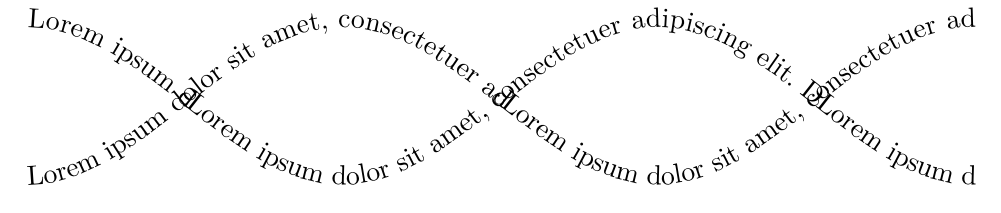
\begin{tikzpicture}
    \path [decorate, decoration={text along path, text={\lorem}}]
    (0,1) cos (2,0);

    \path [decorate, decoration={text along path, text={\lorem}}]
    (2,0) sin (4,-1) cos (6,0) sin (8,1) cos (10,0);

    \path [decorate, decoration={text along path, text={\lorem}}]
    (0,-1) cos (2,0) sin (4,1) cos (6,0);

    \path [decorate, decoration={text along path, text={\lorem}}]
    (6,0) sin (8,-1) cos (10,0) sin (12,1);

    \path [decorate, decoration={text along path, text={\lorem}}]
    (10,0) sin (12,-1);
\end{tikzpicture}
\end{document}

% start:; popl %eax popl; %eax movl $0, %esi; movl $10, %edx; jmp read_arg
% read_arg:; popl %eax; cmpl $0, %eax; je sort; movl $0, %edi; movl $0, %ecx
% store_arg:; movl %ecx, lst(,%esi,4); incl %esi
% read_ch:; movb 0(%eax,%edi), %bl; cmpl $0, %ebx; je store_arg; imul %edx, %ecx; subl $48, %ebx; addl %ebx, %ecx; incl %edi; jmp read_ch
